\documentclass[conference]{IEEEtran}
\usepackage{graphicx}
\usepackage{booktabs}
\usepackage{amsmath}
\usepackage{url}
\usepackage{hyperref}

\title{Restoration and Style-Conditioned Synthesis with Compact Generative Models}
\author{\IEEEauthorblockN{Syed Ashher Majid (23i-0007)}
\IEEEauthorblockA{Department of Computer Science\\FAST NUCES, Islamabad\\Generative AI, CS(A)\\Instructor: Dr Akhtar Jamil}}

\begin{document}
\maketitle

\begin{abstract}
This work studies four related image-to-image systems at a shared 128 $\times$ 128 resolution: a universal pet-image autoencoder, a classifier with corruption-specific restoration experts, a differentiable soft mixture of those experts, and a style-conditioned face-to-sketch generator. The first three tasks use identical Oxford-IIIT Pet splits and reproducible image corruptions; the fourth uses paired FS2K photographs and sketches. Model choice is based on held-out validation data, with official test data reserved for a final evaluation. We provide the source code, experiment records, ONNX models, and a browser application for inspecting predictions.
\end{abstract}

\begin{IEEEkeywords}
image restoration, autoencoder, mixture of experts, conditional GAN, structural similarity
\end{IEEEkeywords}

\section{Introduction}
Image restoration must improve damaged images without unnecessarily altering clean ones. A single autoencoder can learn broad restoration behavior, but corruption-specific networks may exploit more focused training signals. Hard routing chooses one specialist based on a predicted corruption class; its quality can fall when the classifier chooses the wrong branch. Soft routing combines identity and specialist outputs with learned weights, which allows less certain predictions to blend multiple alternatives. We compare these strategies on the same Oxford-IIIT Pet inputs and held-out cases. A separate paired task maps face photographs to three annotated sketch styles.

\section{Related Work}
The Oxford-IIIT Pet dataset introduced by Parkhi \emph{et al.} contains images of 37 cat and dog breeds~\cite{parkhi2012}. Structural similarity (SSIM) compares image structure, luminance and contrast rather than relying only on pixelwise error~\cite{wang2004}. We combine SSIM with mean absolute error (MAE) because the latter provides a direct reconstruction penalty. The mixture-of-experts idea uses a gate to choose or weight specialist predictors~\cite{jacobs1991}. The paired image-to-image method of Isola \emph{et al.} motivates a U-Net generator, conditional patch discriminator, and reconstruction term for sketch synthesis~\cite{isola2017}. FS2K supplies paired photographs and three professionally drawn sketch styles~\cite{fan2022}. Optuna supplies reproducible bounded hyperparameter studies~\cite{akiba2019}.

\section{Data and Evaluation Protocol}
\subsection{Oxford-IIIT Pet}
We preserve the official 3,680-image train/validation partition and 3,669-image test partition. The former is stratified by breed into 2,944 training and 736 validation images with seed 42. All images are converted to RGB and resized to 128 $\times$ 128 using bicubic interpolation. Tasks 1--3 share these exact IDs. Clean training images are damaged dynamically. The four labels are clean, salt-and-pepper noise, Gaussian blur, and black rectangle occlusion. Noise replaces a spatial pixel across all RGB channels, with training probability sampled from 0.02 to 0.15. Blur uses a sampled kernel of size 3, 5, or 7 and Gaussian standard deviation between 0.5 and 2.5. One to three black rectangles cover approximately 10--35\% of the image, with coverage measured as a union of pixels.

For deterministic validation and testing, we store a corruption recipe for every image: one clean case and low, medium, and high severity for each damaged class. This produces 7,360 validation and 36,690 final test cases. Seeds, blur parameters, rectangle coordinates and actual coverage are recorded. The clean target is never modified. Every compared restoration system sees the same damaged inputs.

\subsection{FS2K}
We use the authors' official annotations to pair 1,058 training and 1,046 test photographs with sketches. A style-stratified 15\% validation split of the official training portion gives 899 training and 159 validation pairs, again with seed 42. The annotation's \texttt{style} value, not the photo folder number, supplies the three classes. Paired images receive the same horizontal flip in training. The official test pairs remain untouched until final selection.

\subsection{Metrics and Selection}
For restoration and paired sketch evaluation, we calculate per-image MAE, SSIM, and PSNR. The fixed validation selection score is $0.8\,\mathrm{MAE}+0.2(1-\mathrm{SSIM})$, averaged equally across corruption classes or sketch styles. This score is fixed while training-loss weights vary. Classifier selection uses macro-F1 across the four balanced classes. We separately report clean behavior and each corruption severity, and both overall and style-macro sketch metrics.

\section{Task 1: Universal Autoencoder}
The universal convolutional autoencoder encodes each 128 $\times$ 128 RGB input (49,152 scalar values) into a 48 $\times$ 16 $\times$ 16 latent tensor (12,288 values), a 4:1 compression. It uses no skip connections, so all reconstruction information passes through the bottleneck. Bilinear upsampling and convolutions decode an RGB result. Its training objective is
\begin{equation}
\mathcal{L}_{\mathrm{rec}}=\alpha\lVert \hat{x}-x\rVert_1+(1-\alpha)\bigl(1-\mathrm{SSIM}(\hat{x},x)\bigr).
\end{equation}
We use validation to select architecture width, bottleneck size, learning rate, batch size and $\alpha$ through Optuna. The report will show at least twelve representative cases and four failures using input, target, output and error views.

\section{Task 2: Hard Routing}
A four-class convolutional classifier predicts clean, noise, blur or occlusion. Balanced mini-batches contain equal counts of every class, and cross-entropy trains the classifier. Three independent autoencoders are each trained on one damage type using MAE and SSIM. Predicted clean images use an exact identity bypass. We compare an oracle, which chooses the true branch, with the deployed route, which uses the classifier prediction. Their difference isolates routing errors from specialist restoration quality.

\section{Task 3: Soft Mixture of Experts}
The soft model initializes its gate and three experts from the trained Task 2 checkpoints. Identity is branch 0. For input $z$, the gate returns four normalized weights $w_i(z)$, and the output is
\begin{equation}
\hat{x}=w_0(z)z+\sum_{i=1}^{3} w_i(z)E_i(z),\qquad \sum_{i=0}^{3}w_i(z)=1.
\end{equation}
Initially the experts are frozen while the gate adapts. Joint fine-tuning then updates experts with a smaller learning rate. The loss combines reconstruction, gate cross-entropy, and a batch-level balance penalty. We examine average weights by true class and severity to identify useful specialization or branch collapse.

\section{Task 4: Conditional Face-to-Sketch GAN}
The generator receives a normalized photograph and a learned embedding of one of three FS2K style labels. A compact U-Net with skip connections produces a three-channel sketch. A PatchGAN discriminator receives the photograph, real or generated sketch, and its own learned style embedding. We alternate discriminator and generator updates with binary cross-entropy adversarial loss; the generator also minimizes a weighted paired $\ell_1$ term. Optuna searches learning rates, batch size, width, dropout, style-embedding size, and reconstruction weight. The best configuration is trained beyond the short search trials before final test evaluation.

\section{Implementation and Reproducibility}
Training uses PyTorch, fixed seeds, saved dataset manifests, resume checkpoints, and local MLflow experiment records. The final model graphs are exported to ONNX and checked against PyTorch output numerically before FastAPI inference. A React and Tailwind browser interface, designed in Google Stitch, exposes all four workspaces. Docker Compose starts the frontend and CPU inference backend with one command. The Git repository excludes raw datasets, secrets, virtual environments, and mutable experiment stores.

\begin{figure}[t]
\centering
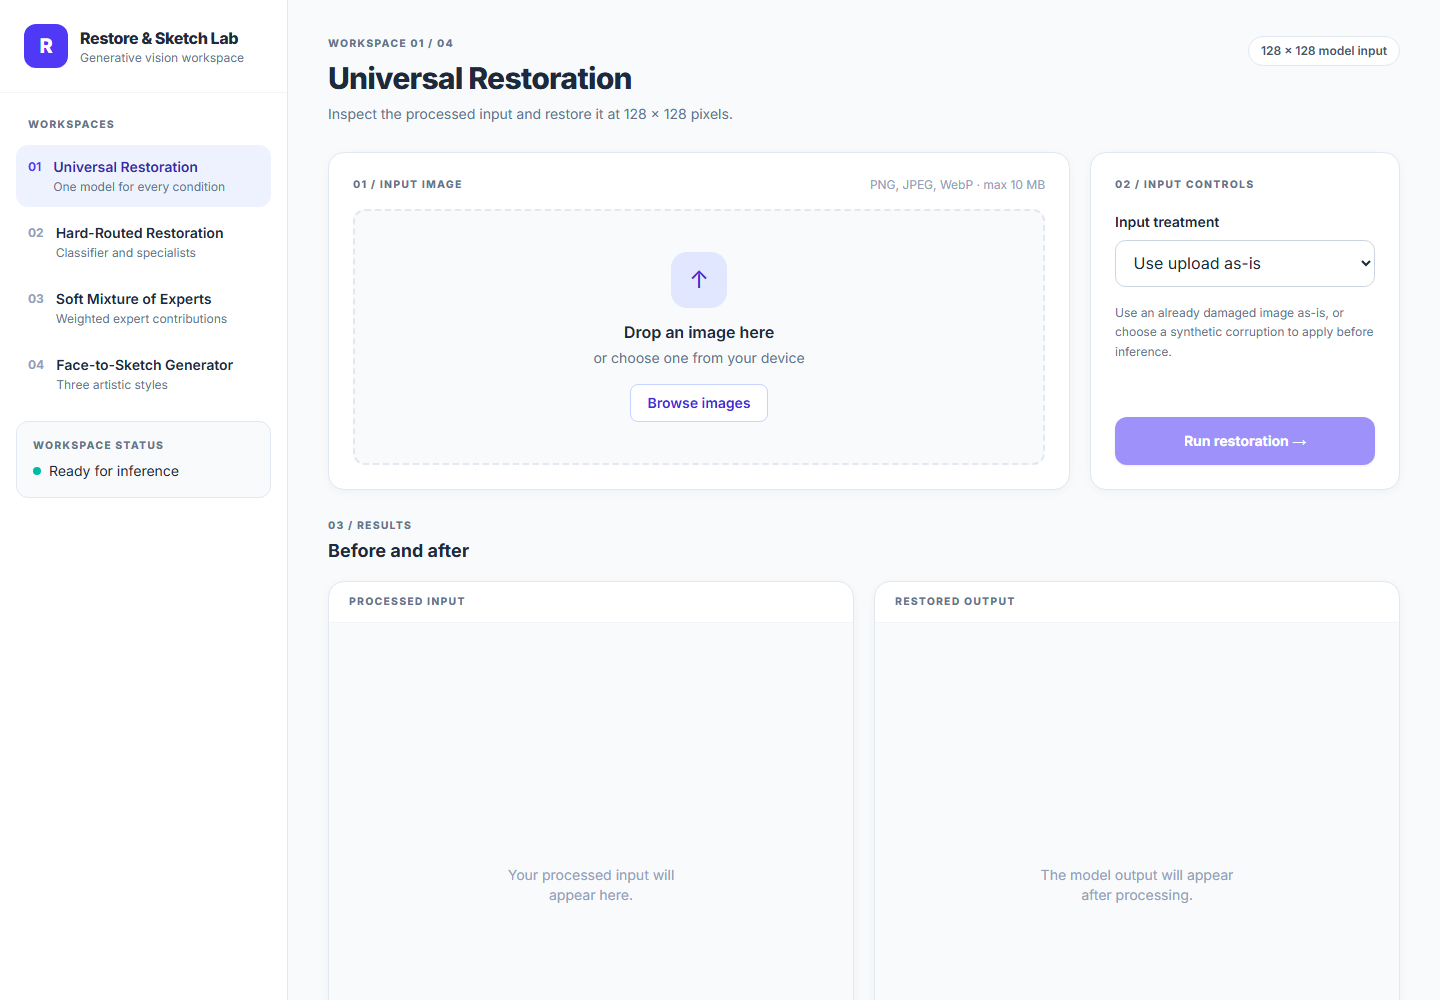
\includegraphics[width=\columnwidth]{figures/application_dashboard.png}
\caption{The browser interface showing the universal restoration workspace. Workspace availability is reported by the inference backend.}
\label{fig:application}
\end{figure}

\section{Experimental Results}
\begin{table}[t]
\centering
\caption{Held-out FS2K test results for the selected local conditional GAN (1,046 paired images). The style-macro row weights each style equally.}
\label{tab:fs2k}
\begin{tabular}{lrrrr}
\toprule
Style & $n$ & MAE $\downarrow$ & SSIM $\uparrow$ & PSNR $\uparrow$ \\
\midrule
1 & 619 & 0.0871 & 0.4982 & 16.57 \\
2 & 381 & 0.1662 & 0.3594 & 11.67 \\
3 & 46 & 0.0724 & 0.5724 & 17.73 \\
\midrule
Overall & 1,046 & 0.1153 & 0.4509 & 14.83 \\
Style macro & -- & 0.1085 & 0.4767 & 15.32 \\
\bottomrule
\end{tabular}
\end{table}

The FS2K model was selected by validation and evaluated once on the held-out test split. Style 2 has the largest reconstruction error, while style 3 has the lowest. These scores measure similarity to the annotated paired sketch, not artistic preference. Figure~\ref{fig:fs2k-samples} shows examples across all three styles, and Figure~\ref{fig:fs2k-failures} shows the lowest-SSIM test cases.

\begin{figure}[t]
\centering
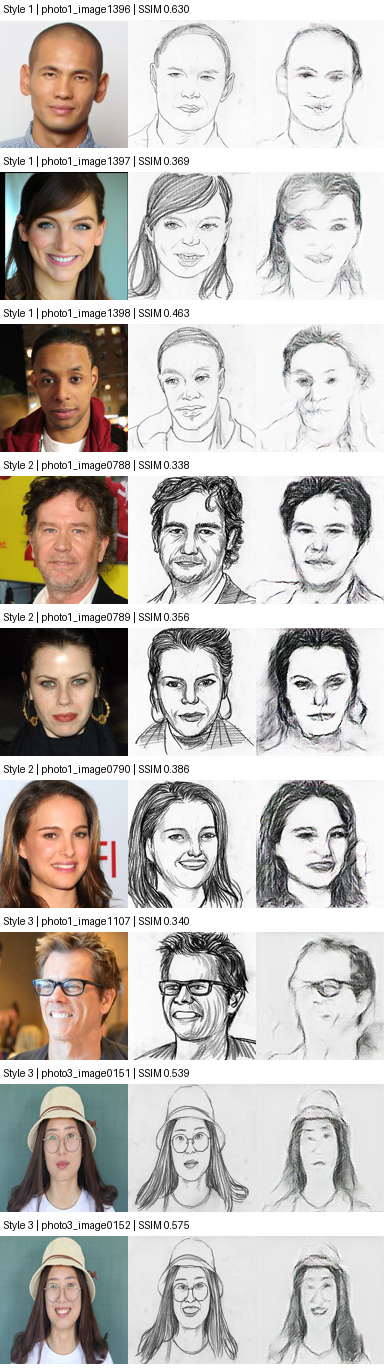
\includegraphics[width=\columnwidth]{figures/task4_samples.png}
\caption{FS2K test examples: input photograph, paired target, generated sketch.}
\label{fig:fs2k-samples}
\end{figure}

\begin{figure}[t]
\centering
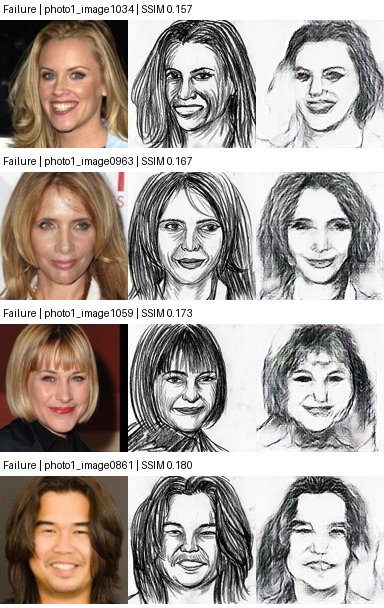
\includegraphics[width=\columnwidth]{figures/task4_failures.png}
\caption{Four held-out FS2K cases with the lowest structural similarity.}
\label{fig:fs2k-failures}
\end{figure}

\begin{table}[t]
\centering
\caption{Task 1 universal autoencoder on the untouched Oxford-IIIT Pet test set. Each row contains 3,669 images.}
\label{tab:task1}
\begin{tabular}{llrrr}
\toprule
Condition & Severity & MAE $\downarrow$ & SSIM $\uparrow$ & PSNR $\uparrow$ \\
\midrule
Clean & none & 0.0355 & 0.8068 & 25.84 \\
Salt-and-pepper & low & 0.0355 & 0.8006 & 25.88 \\
Salt-and-pepper & medium & 0.0363 & 0.7873 & 25.74 \\
Salt-and-pepper & high & 0.0390 & 0.7602 & 25.21 \\
Gaussian blur & low & 0.0345 & 0.8088 & 26.16 \\
Gaussian blur & medium & 0.0347 & 0.7888 & 26.11 \\
Gaussian blur & high & 0.0400 & 0.7174 & 24.80 \\
Occlusion & low & 0.0420 & 0.7595 & 23.64 \\
Occlusion & medium & 0.0486 & 0.7132 & 22.15 \\
Occlusion & high & 0.0599 & 0.6414 & 20.37 \\
\bottomrule
\end{tabular}
\end{table}

The selected Task 1 configuration used learning rate $1.03\times10^{-4}$, batch size 16, 24 base channels, a 48-channel bottleneck, and $\alpha=0.526$. The bounded search completed three trials; the selected trial's short-run validation objective was 0.1421. A matched four-epoch follow-up varied only autoencoder dropout: 0.0 achieved validation objective 0.1438 versus 0.1488 at dropout 0.2, on the same 128 validation IDs and 75 training steps per epoch. This short comparison favors no dropout but does not prove the ranking would persist over a full training run. Final training reached epoch 35, with best full-validation objective 0.07750 at epoch 33. On the 36,690 fixed test cases, high occlusion is the most difficult condition (MAE 0.0599, SSIM 0.6414), while low blur is the strongest (MAE 0.0345, SSIM 0.8088). This gap is consistent with the information loss from large masked regions; the remaining errors are visible in the example and failure panels.

\begin{figure}[t]
\centering
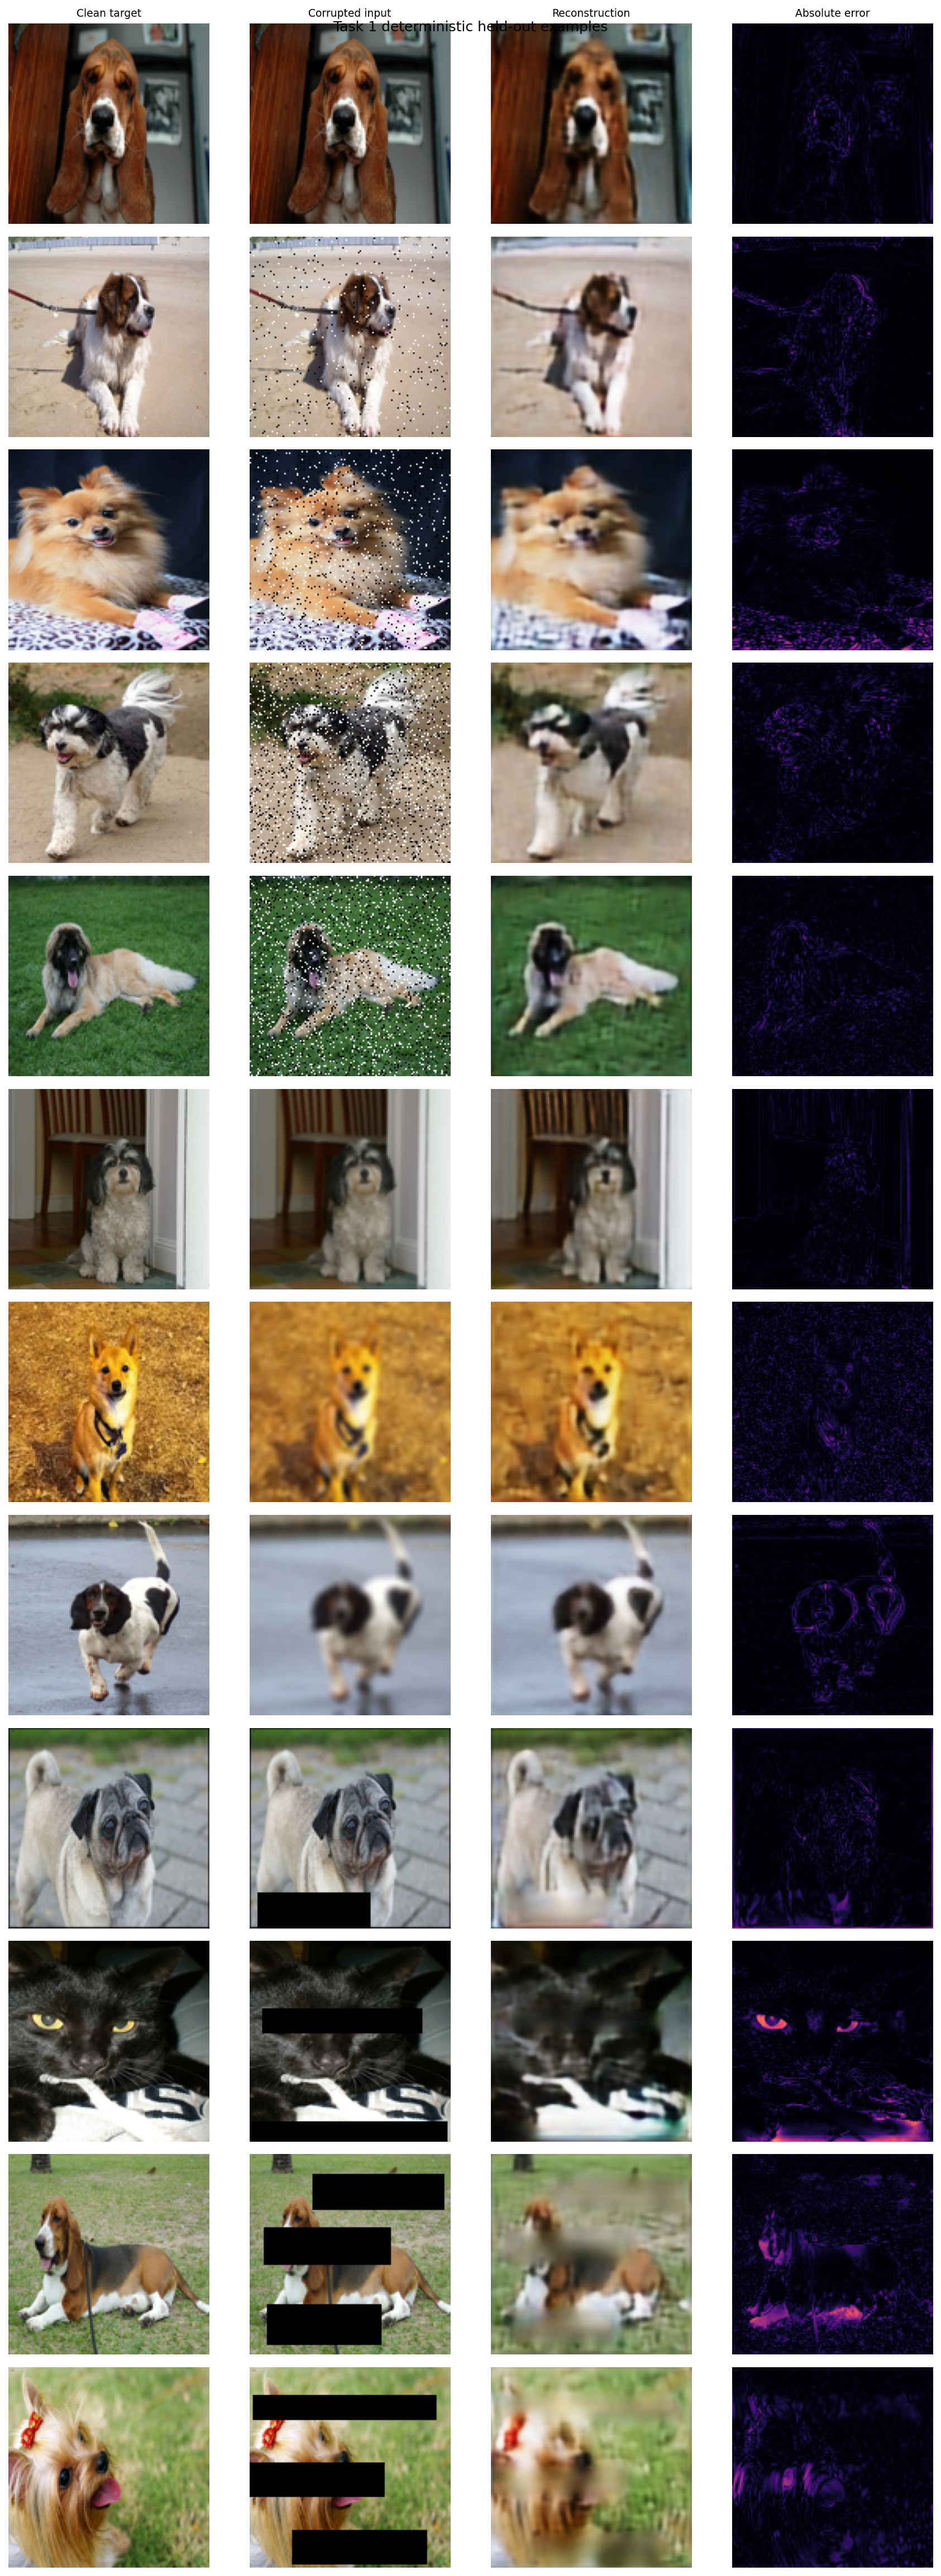
\includegraphics[width=\columnwidth]{figures/task1_examples.png}
\caption{Twelve Task 1 test cases with clean target, corrupted input, reconstruction, and absolute error map.}
\label{fig:task1-examples}
\end{figure}

\begin{figure}[t]
\centering
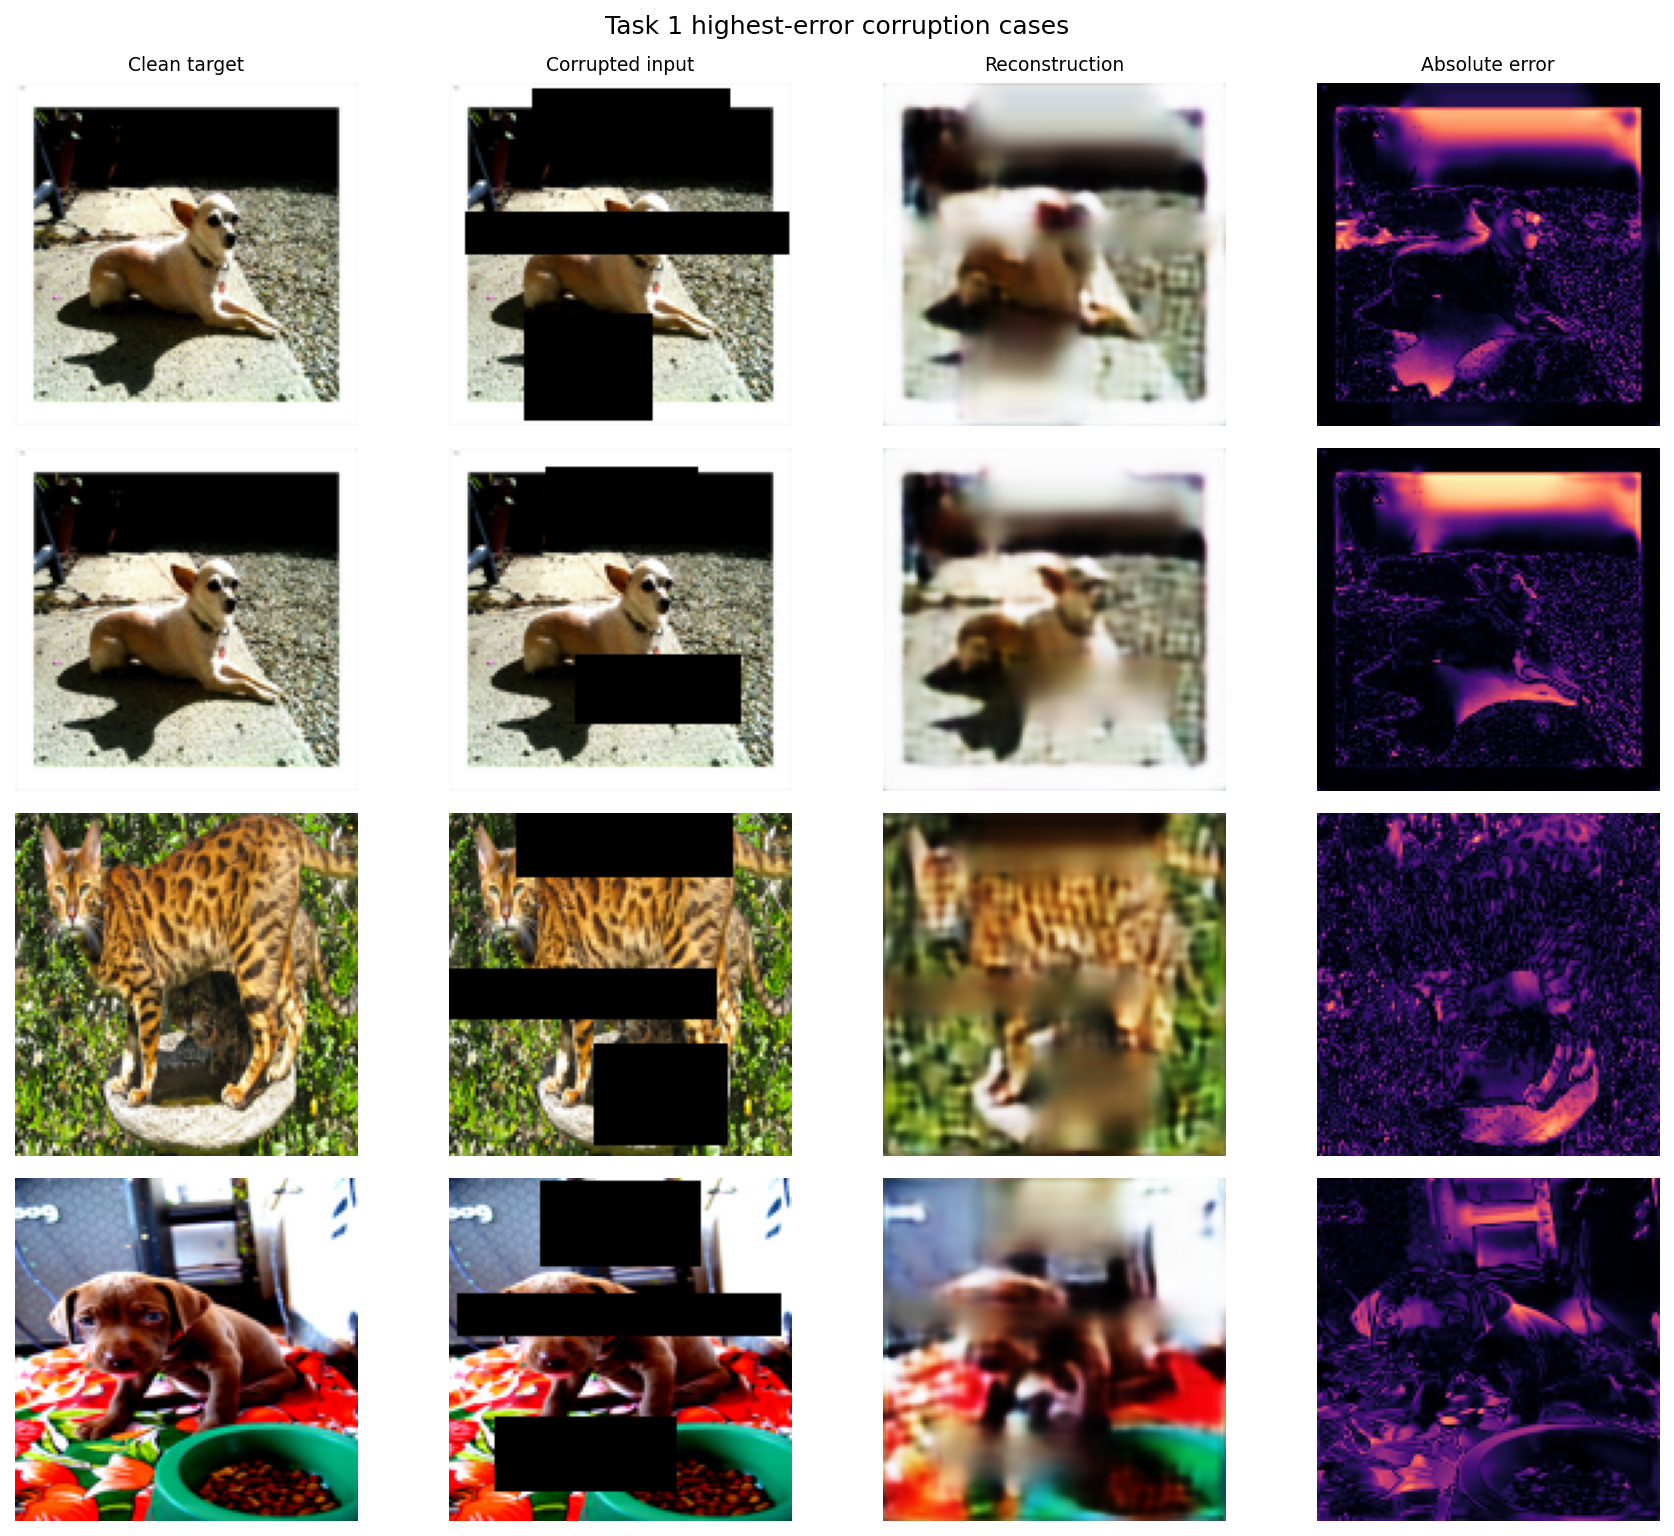
\includegraphics[width=\columnwidth]{figures/task1_failures.png}
\caption{Four highest-error Task 1 test cases selected from the fixed corruption manifest.}
\label{fig:task1-failures}
\end{figure}

Task 2's selected classifier checkpoint (epoch 22) was assessed on the 7,360 deterministic validation cases. It reached 99.58\% accuracy and 0.9931 macro-F1. The remaining errors are concentrated in clean-versus-blur and occlusion-versus-clean confusions; the specialist routing results are reported separately after expert training.

\begin{table}[t]
\centering
\caption{Task 2 classifier validation results.}
\label{tab:classifier-validation}
\begin{tabular}{lrrrr}
\toprule
Class & Support & Precision & Recall & F1 \\
\midrule
Clean & 736 & 0.9719 & 0.9878 & 0.9798 \\
Salt-and-pepper & 2,208 & 0.9991 & 1.0000 & 0.9995 \\
Gaussian blur & 2,208 & 0.9986 & 0.9973 & 0.9980 \\
Occlusion & 2,208 & 0.9977 & 0.9928 & 0.9952 \\
\midrule
Macro average & 7,360 & 0.9918 & 0.9945 & 0.9931 \\
\bottomrule
\end{tabular}
\end{table}

\begin{figure}[t]
\centering
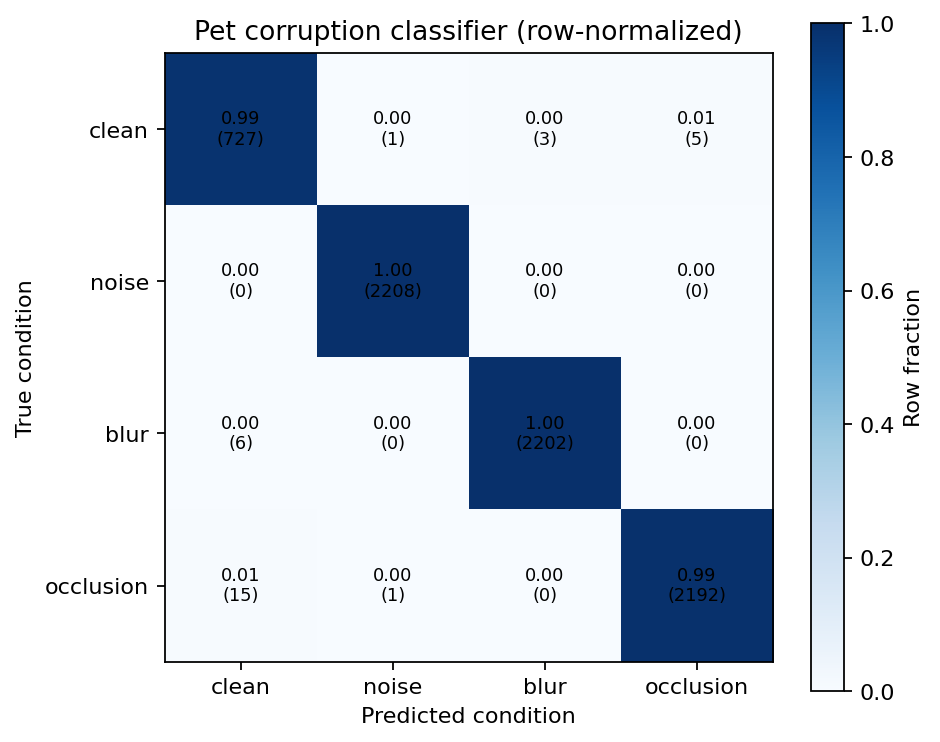
\includegraphics[width=0.76\columnwidth]{figures/task2_classifier_confusion.png}
\caption{Task 2 corruption classifier row-normalized validation confusion matrix; counts are annotated in parentheses.}
\label{fig:task2-classifier-confusion}
\end{figure}


\section{Discussion and Limitations}
The Task 1 results show a consistent severity effect for spatially destructive inputs: MAE rises from 0.0420 at low occlusion to 0.0599 at high occlusion, while SSIM falls from 0.7595 to 0.6414. High noise and blur also reduce structure scores, but remain easier than large masked regions. On clean inputs the autoencoder still changes pixels (MAE 0.0355), unlike Task 2's explicit identity bypass; this is a measured limitation of a single shared reconstruction path. The Task 2 classifier reached 0.9931 validation macro-F1, but this validation result alone does not establish routed test performance; the held-out oracle-versus-predicted comparison remains necessary to attribute errors to routing or expert quality.

For FS2K, the paired-test error is largest for style 2 (MAE 0.1662, SSIM 0.3594). Style 3 has the best measured scores but only 46 test examples, compared with 619 and 381 for styles 1 and 2, respectively. The style-macro metrics therefore complement, rather than replace, the overall average. Scores measure agreement with the annotated paired sketch, not subjective artistic quality; counterfactual targets for the other two styles are unavailable.

\section{Conclusion}
The final conclusion will reflect the recorded held-out results and identified failure cases.

\appendices
\section{AI Assistance and Verification}
AI assistance was used to organize the assignment plan; draft implementation code, interface prompts, and report text. The author verified dataset split counts and provenance, inspected generated UI output, ran automated and GPU checks, reviewed numerical results and failures, and retained responsibility for technical claims. AI-generated code and prose were revised where checks exposed errors. The repository records design prompts and experiment configurations for auditability.

\section{Demonstration and Artifacts}
The final YouTube demonstration link and model download locations will be inserted after the outputs are verified.

\begin{thebibliography}{9}
\bibitem{parkhi2012} O. M. Parkhi, A. Vedaldi, A. Zisserman, and C. V. Jawahar, ``Cats and Dogs,'' in \emph{Proc. CVPR}, 2012. [Online]. Available: \url{https://www.robots.ox.ac.uk/~vgg/publications/2012/parkhi12a/}
\bibitem{wang2004} Z. Wang, A. C. Bovik, H. R. Sheikh, and E. P. Simoncelli, ``Image quality assessment: From error visibility to structural similarity,'' \emph{IEEE Trans. Image Process.}, vol. 13, no. 4, pp. 600--612, 2004. [Online]. Available: \url{https://ece.uwaterloo.ca/~z70wang/research/ssim/}
\bibitem{jacobs1991} R. A. Jacobs, M. I. Jordan, S. J. Nowlan, and G. E. Hinton, ``Adaptive mixtures of local experts,'' \emph{Neural Computation}, vol. 3, no. 1, pp. 79--87, 1991.
\bibitem{isola2017} P. Isola, J.-Y. Zhu, T. Zhou, and A. A. Efros, ``Image-to-image translation with conditional adversarial networks,'' in \emph{Proc. CVPR}, 2017. [Online]. Available: \url{https://openaccess.thecvf.com/content_cvpr_2017/html/Isola_Image-To-Image_Translation_With_CVPR_2017_paper.html}
\bibitem{fan2022} D.-P. Fan \emph{et al.}, ``Facial-sketch synthesis: A new challenge,'' 2022. [Online]. Available: \url{https://github.com/DengPingFan/FS2K}
\bibitem{akiba2019} T. Akiba, S. Sano, T. Yanase, T. Ohta, and M. Koyama, ``Optuna: A next-generation hyperparameter optimization framework,'' in \emph{Proc. KDD}, 2019. [Online]. Available: \url{https://arxiv.org/abs/1907.10902}
\end{thebibliography}

\end{document}

